\documentclass[11pt]{article}
\usepackage[margin=0.9in]{geometry}
\usepackage[T1]{fontenc}
\usepackage{lmodern}
\usepackage{microtype}
\usepackage{graphicx}
\usepackage{booktabs}
\usepackage{amsmath}
\usepackage[font=small,labelfont=it]{caption}
\usepackage[hidelinks]{hyperref}
\newcommand{\nLc}{0.363}
\newcommand{\nLinf}{0.061}
\newcommand{\nLinfSteps}{15.6}
\newcommand{\nSSIM}{0.9977}
\newcommand{\nPSNR}{45.9}
\newcommand{\nLPIPS}{0.00019}
\newcommand{\nQueries}{4956}
\newcommand{\nTotalQueries}{4\,956\,199}
\newcommand{\nFixed}{2}
\newcommand{\nGtEight}{734}
\newcommand{\nGtSixteen}{405}
\newcommand{\nLinfMedian}{14}
\newcommand{\nLinfMax}{54}
\newcommand{\nMedLc}{0.325}
\newcommand{\nMaxLc}{1.38}
\newcommand{\nMinLc}{0.007}
\newcommand{\nPninety}{0.68}
\newcommand{\nBaseLc}{4.64}
\newcommand{\nTopA}{frog}
\newcommand{\nTopAn}{258}
\newcommand{\nTopB}{bird}
\newcommand{\nTopBn}{228}
\newcommand{\nTopC}{cat}
\newcommand{\nTopCn}{119}
\newcommand{\nBottomA}{horse}
\newcommand{\nBottomAn}{18}
\newcommand{\nBottomB}{automobile}
\newcommand{\nBottomBn}{21}
\newcommand{\nStudyBaseLc}{0.288}
\newcommand{\nLowA}{0.467}
\newcommand{\nLowB}{0.892}
\newcommand{\nMulti}{0.295}
\newcommand{\nTexA}{0.309}
\newcommand{\nTexB}{0.365}
\newcommand{\nMarginZeroJit}{34}
\newcommand{\nMarginFiveJit}{94}
\newcommand{\nMarginZeroHolds}{48}
\newcommand{\nMarginFiveLc}{0.379}
\newcommand{\nLHbaaa}{0.727}
\newcommand{\nLHcaaa}{0.464}
\newcommand{\nLHfaaa}{0.288}
\newcommand{\nLSbaaa}{0.833}
\newcommand{\nLScaaa}{0.522}
\newcommand{\nLSfaaa}{0.356}
\newcommand{\nLCbaaa}{1.083}
\newcommand{\nLCcaaa}{0.832}
\newcommand{\nLCfaaa}{0.682}
   % every number below comes from numbers.tex / tables.tex, written by make_figures.py
\newcommand{\tabMain}{\begin{tabular}{lrrrrrr}\toprule
 success & L2 & L$_\infty$ & SSIM & PSNR (dB) & LPIPS & queries\\\midrule
1000/1000 & 0.363 & 0.061 & 0.9977 & 45.9 & 0.00019 & 4956\\\bottomrule\end{tabular}}
\newcommand{\tabCompare}{\begin{tabular}{lrrrrr}\toprule
 & \multicolumn{3}{c}{mean L2 at budget} & \multicolumn{2}{c}{at 5000}\\
\cmidrule(lr){2-4}\cmidrule(lr){5-6}
 attack & 1000 & 2000 & 5000 & L$_\infty$ & SSIM\\\midrule
HSJA & \textbf{0.727} & \textbf{0.464} & \textbf{0.288} & 0.025 & 0.9969\\
SurFree & 0.833 & 0.522 & 0.356 & 0.035 & 0.9955\\
CGBA & 1.083 & 0.832 & 0.682 & 0.060 & 0.9851\\
\bottomrule\end{tabular}}
\newcommand{\tabReach}{\begin{tabular}{lrrrr}\toprule
 attack & L2 $\le$ 2 & $\le$ 1 & $\le$ 0.5 & $\le$ 0.25\\\midrule
HSJA & 325 & 725 & 1387 & 3975\\
SurFree & 175 & 562 & 1450 & $>$5000\\
CGBA & 300 & 925 & $>$5000 & $>$5000\\
\bottomrule\end{tabular}}
\newcommand{\tabStudy}{\begin{tabular}{lrrrrrl}\toprule
 change & L2 & L$_\infty$ & SSIM & holds & jitter & kept\\\midrule
HSJA, 1\% margin & 0.288 & 0.025 & 0.9969 & 50/50 & 76\% & yes\\
low-frequency probes, 16$\times$16 DCT & 0.467 & 0.046 & 0.9929 & 50/50 & 76\% & no\\
low-frequency probes, 8$\times$8 DCT & 0.892 & 0.072 & 0.9794 & 50/50 & 82\% & no\\
best of several starting points & 0.295 & 0.027 & 0.9970 & 50/50 & 80\% & no\\
texture-weighted probes, $p=0.5$ & 0.309 & 0.037 & 0.9978 & 50/50 & 78\% & no\\
texture-weighted probes, $p=1$ & 0.365 & 0.058 & 0.9979 & 50/50 & 76\% & yes\\
margin 0\% & 0.362 & 0.058 & 0.9979 & 48/50 & 34\% & no\\
margin 2\% & 0.369 & 0.059 & 0.9979 & 50/50 & 82\% & no\\
margin 5\% & 0.379 & 0.061 & 0.9977 & 50/50 & 94\% & yes\\
\bottomrule\end{tabular}}

\graphicspath{{figures/}}
\setlength{\parskip}{0.4em}
\setlength{\textfloatsep}{10pt plus 2pt minus 2pt}
\setlength{\floatsep}{8pt plus 2pt minus 2pt}
\setlength{\parindent}{0pt}

\title{Hard-label black-box attacks on a CIFAR-10 classifier:\\ a research log}
\author{The FOOLML team}
\date{\today}

\begin{document}
\maketitle

\section{Problem setting}

We were handed a trained CNN for CIFAR-10 \cite{krizhevsky2009} and 1000 test images, 100 per class. The model takes a normalised 32$\times$32 colour image and returns one class index. That is all it returns. We could query it as often as we liked, but we were not allowed to look at weights, activations, logits, probabilities or gradients, and a submission is disqualified if it does. The task is to save one adversarial PNG per clean image, named \texttt{cat\_5.png} $\to$ \texttt{cat\_5\_adv.png}, such that the model gets as many of them wrong as possible while the change stays hard to see. The organisers' scoring splits evenly between attack success rate and imperceptibility, with ties broken by fewer queries and a larger change in the model's confidence.

The model classifies all 1000 clean images correctly. Two constraints shaped almost every later choice. First, the attack sees one label per query, which is the decision-based setting of \cite{brendel2018}, so any gradient-like quantity has to be estimated from yes/no answers. Second, the organisers did not say which imperceptibility metric they use. We report L2, L$_\infty$, SSIM, PSNR and LPIPS \cite{zhang2018lpips} throughout, and we made choices on L2 and SSIM because those were what we had been told to watch. If the hidden metric is closer to L$_\infty$ than to L2, one of our decisions (texture weighting, section~\ref{sec:tried}) may have gone the wrong way, and we flag it where it matters.

All model access goes through one small wrapper, \texttt{QueryModel}. It takes images in $[0,1]$, normalises them, returns labels, and increments a per-image counter. Every attack in this report calls the wrapper and nothing else, so the query counts we quote include everything: starting-point search, the attack proper, and the verification queries.

\section{Method}

Figure~\ref{fig:arch} shows the pipeline. The attack is untargeted and works in $L_2$. We start from some image the model gets wrong, however far away, and move it toward the clean image while keeping it wrong, so the final image sits just across the decision boundary.

\begin{figure}[tbp]
\centering
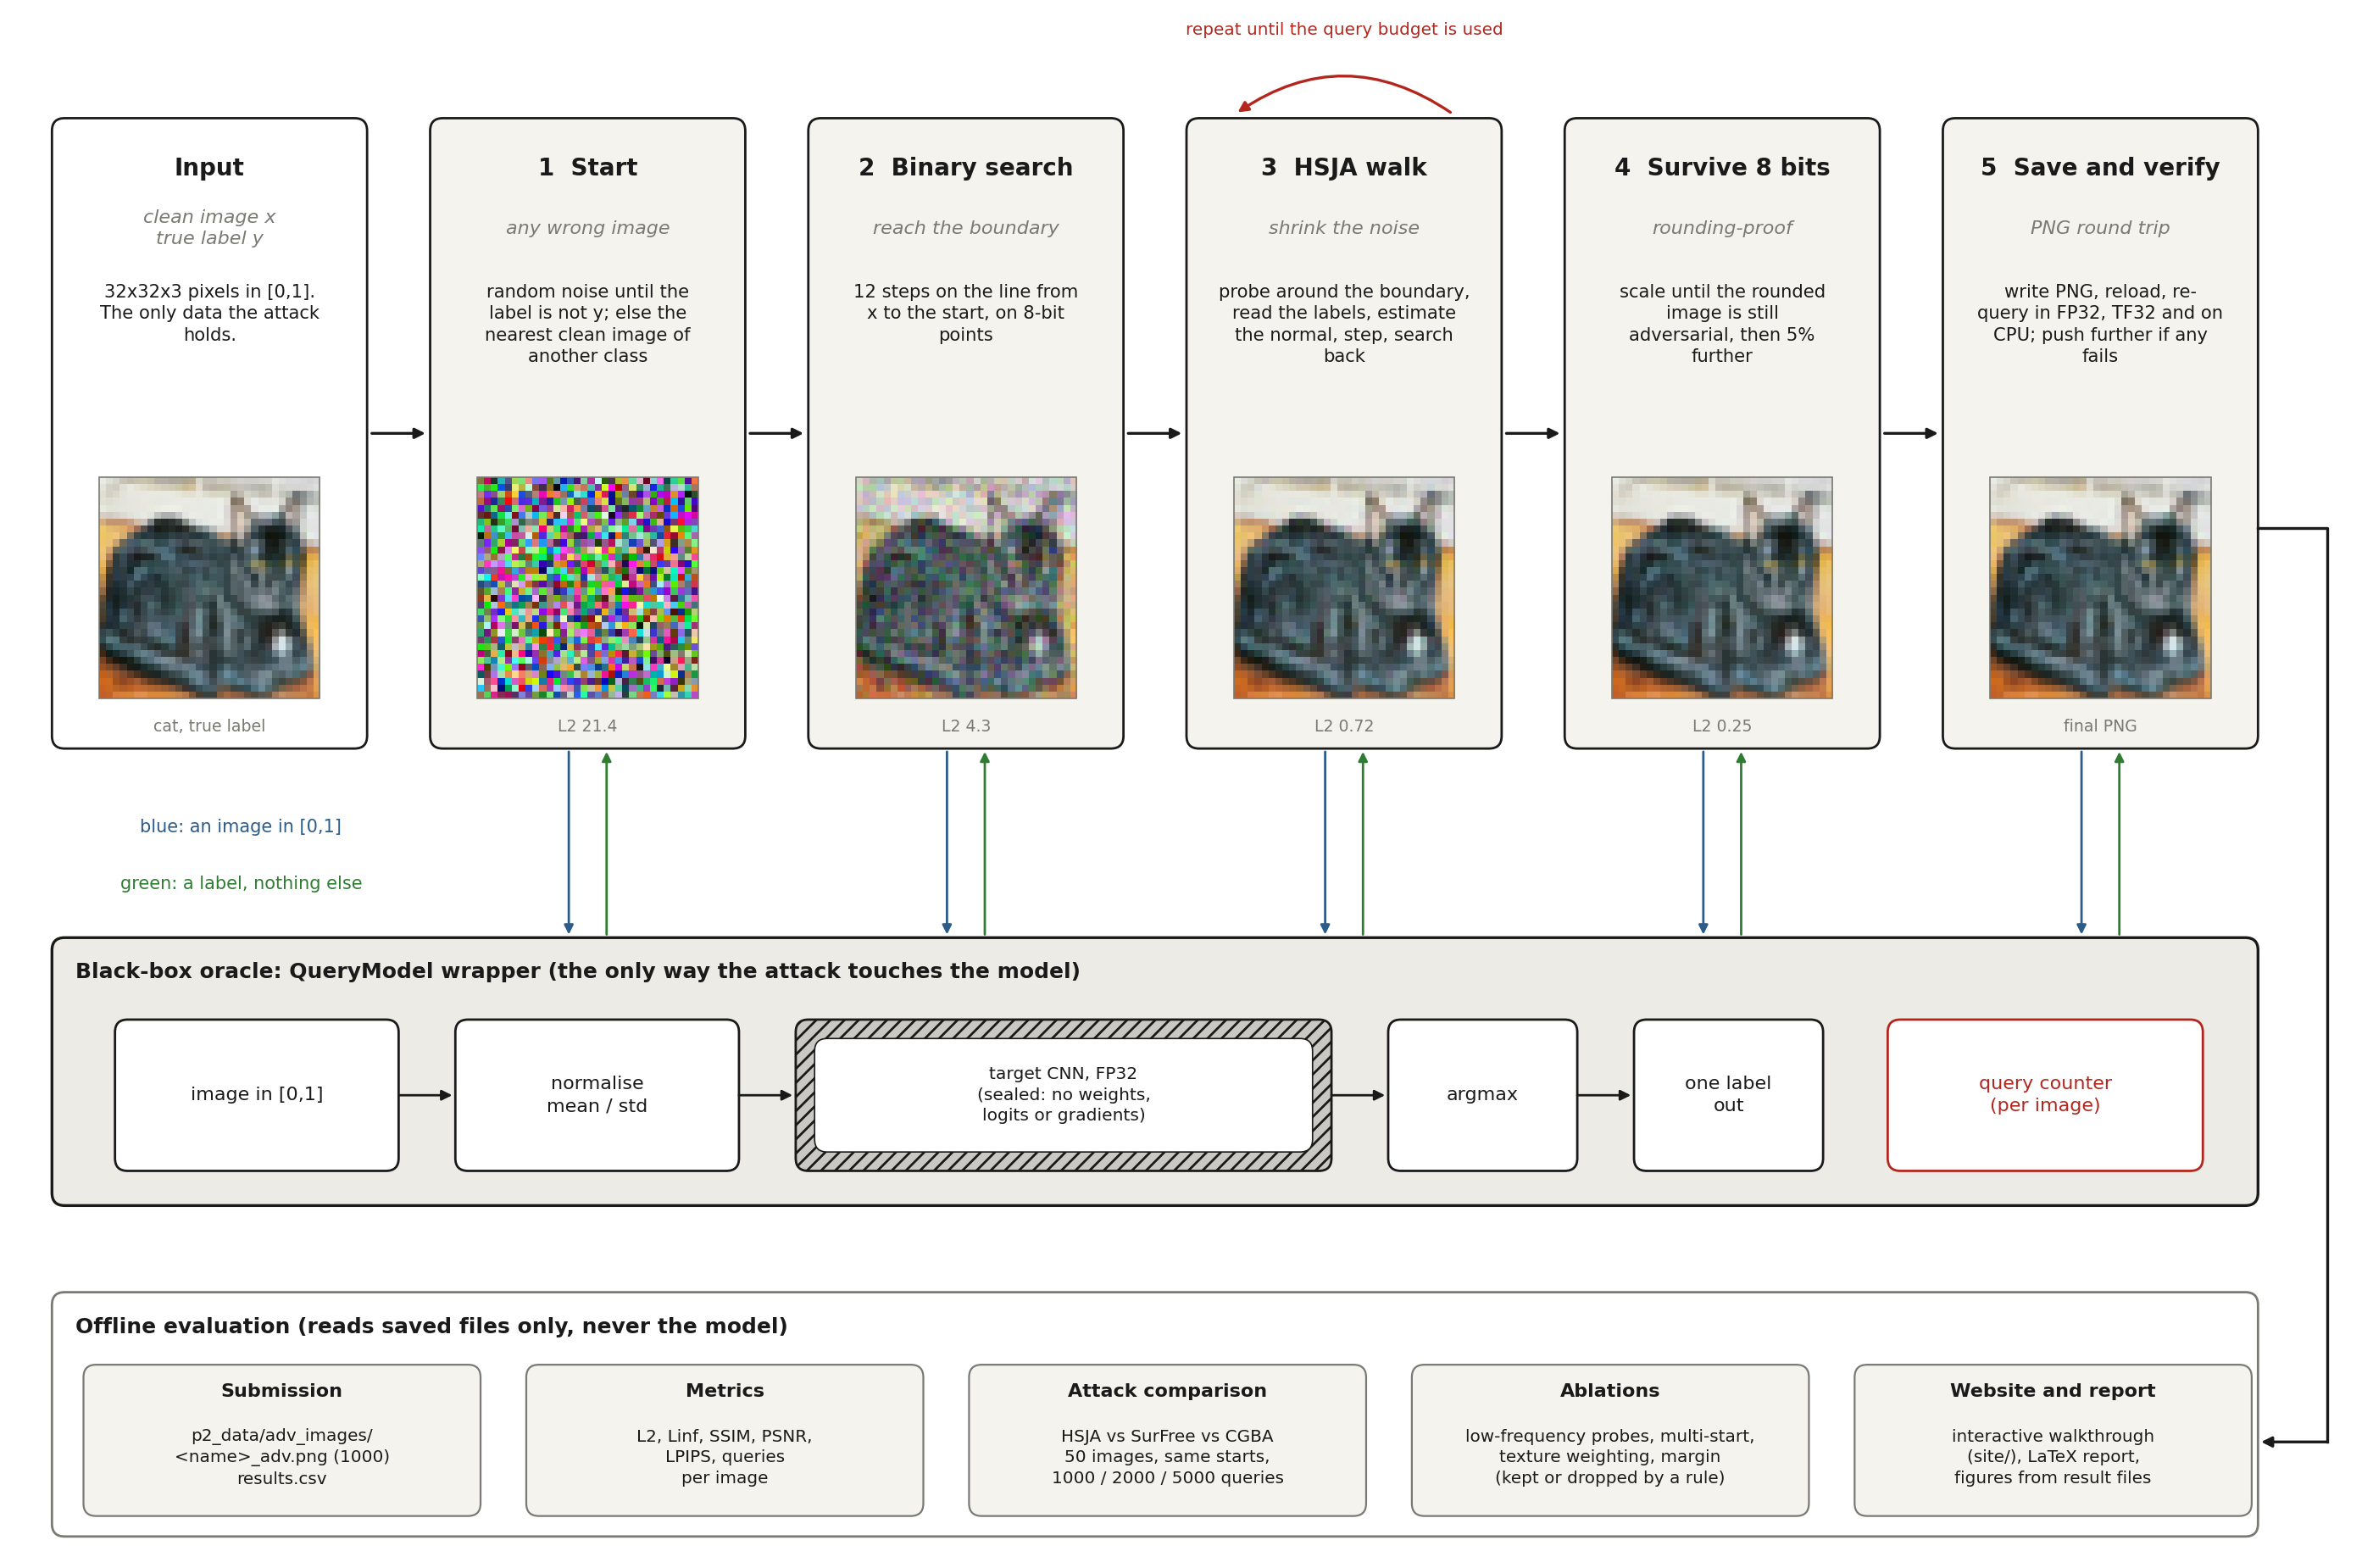
\includegraphics[width=0.8\textwidth]{architecture.png}
\caption{The attack and its surroundings. The six boxes on top are the pipeline, with real intermediate images for \texttt{cat\_7}. Every arrow into the model passes through the query wrapper, which returns one label and counts the query. The bottom row only reads saved files. Note the model box is sealed: nothing leaves it except the label.}
\label{fig:arch}
\end{figure}

\paragraph{Start and binary search.} We draw uniform noise until the model calls it something other than the true class, trying at most ten times, and fall back to the nearest clean image of another predicted class if none works. Then we binary-search for twelve steps along the line from the clean image to this start, testing only 8-bit quantised points. This lands on the boundary at a cost of about 14 queries. The mean L2 of the resulting images over our 50 study images is \nBaseLc, which is the number everything else has to beat.

\paragraph{HopSkipJumpAttack.} The main work is done by HopSkipJumpAttack \cite{chen2020hsja}, which we implemented from the paper and the authors' code so that it could only touch the wrapper. At a boundary point $b$ it draws $n = 100\sqrt{t}$ random directions $u_i$ at iteration $t$, queries $b + \delta u_i$, and scores each answer $+1$ if the label is wrong and $-1$ otherwise. The mean of the scores times the directions, after subtracting the mean score, estimates the normal to the boundary. We take a geometric step along it, halving the step until the point is adversarial, and binary-search back to the boundary (figure~\ref{fig:loop}). Each pass makes the perturbation a bit smaller.

\begin{figure}[tbp]
\centering
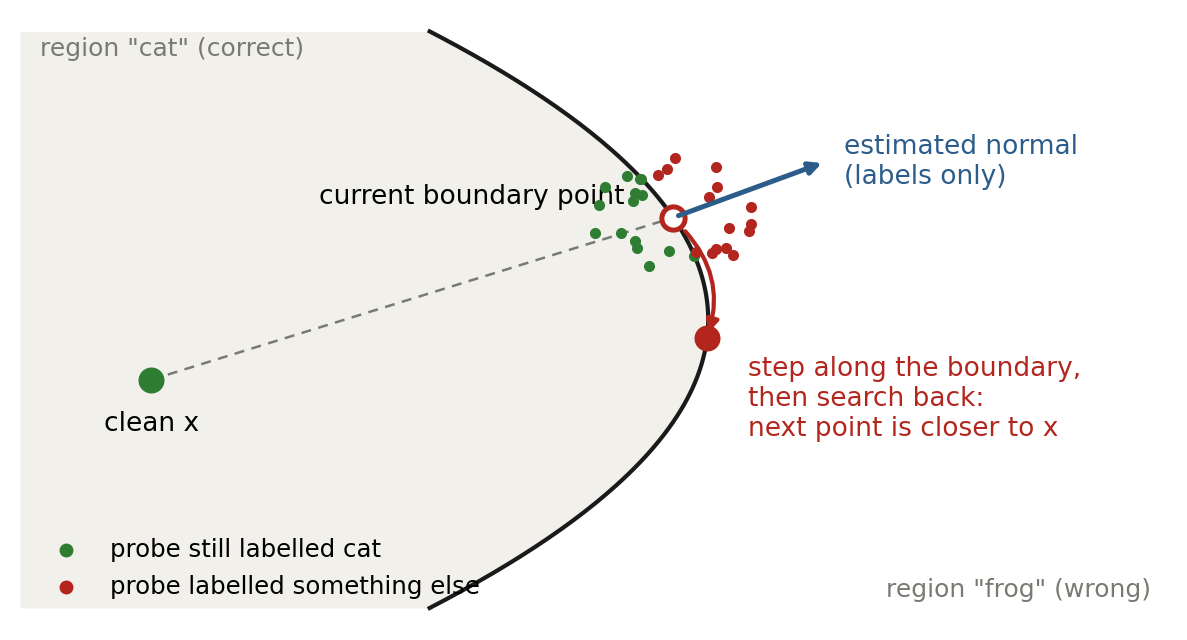
\includegraphics[width=0.44\textwidth]{hsja_loop.png}
\caption{One HSJA iteration, drawn as a sketch and not from data. Probes around the boundary point return only a label. Their average direction estimates the normal, and a step plus a short binary search yields a boundary point that is closer to the clean image.}
\label{fig:loop}
\end{figure}

\paragraph{Texture-weighted probes.} In the final configuration the random directions are multiplied element-wise by the local standard deviation of the clean image (3$\times$3 window, grey-scale, divided by its mean), so more of the perturbation lands on edges and textured regions. We kept this on an SSIM-first rule; it costs L2, as section~\ref{sec:tried} shows.

\paragraph{Surviving the PNG.} HSJA works in floating point, but the submission is an 8-bit PNG. For some images HSJA reaches a perturbation with L2 around 0.001, which is smaller than a single 1/255 step on one pixel, and rounding erases it. After HSJA we therefore scale the perturbation outward along the ray from the clean image until the \emph{rounded} image is still adversarial, refine this with four binary-search steps, and push 5\% further as a safety margin.

\paragraph{Save and verify.} We write the PNGs, reload them, and query again. Anything that is not misclassified in full FP32, with TF32 enabled at batch size 1 and at full batch, and on the CPU is pushed further along the ray and re-saved. In the final run \nFixed{} images needed this. The whole run takes about 24 minutes for 1000 images on an RTX 4070.

\section{What we tried}
\label{sec:tried}

\subsection{Three published attacks}

We implemented HSJA, SurFree \cite{maho2021surfree} and CGBA \cite{reza2023cgba} and ran all three on 50 images, five per class, from the same starting points and with the same per-image budgets of 1000, 2000 and 5000 queries. The budget includes the starting-point queries. All nine runs fooled all 50 images, so the comparison is entirely about how small the perturbation is.

\begin{table}[tbp]
\centering
\begin{minipage}[t]{0.53\textwidth}\centering\small\tabCompare\end{minipage}\hfill
\begin{minipage}[t]{0.44\textwidth}\centering\small\tabReach\end{minipage}
\caption{Left: mean L2 on the 50 study images at three query budgets, then L$_\infty$ and SSIM at 5000 queries. HSJA is best in every column. For reference the starting point alone has L2 \nBaseLc. Right: median number of queries before the best L2 so far drops below each threshold. Images that never get there count as above 5000, so a median of $>$5000 means more than half the images did not.}
\label{tab:compare}
\end{table}

HSJA gave the smallest perturbation at every budget (table~\ref{tab:compare}), and the margin grows with the budget: at 5000 queries CGBA is more than twice as far from the clean image as HSJA. SurFree behaves differently early on. Figure~\ref{fig:curve} and the right half of table~\ref{tab:compare} show that it gets to L2 $\le$ 1 in a median of 562 queries against 725 for HSJA, and then falls behind. We did not investigate why; our guess is that SurFree's random low-frequency search works while the perturbation is large and loses out once the boundary has to be followed closely.

CGBA improves slowly and is still at \nLCfaaa{} after 5000 queries, against \nLCcaaa{} after 2000. We used the reference settings for CIFAR-10 and ported the code ourselves, so a porting error is quite possible and we would not claim the method is weak on this task on the strength of our numbers.

\begin{figure}[tbp]
\centering
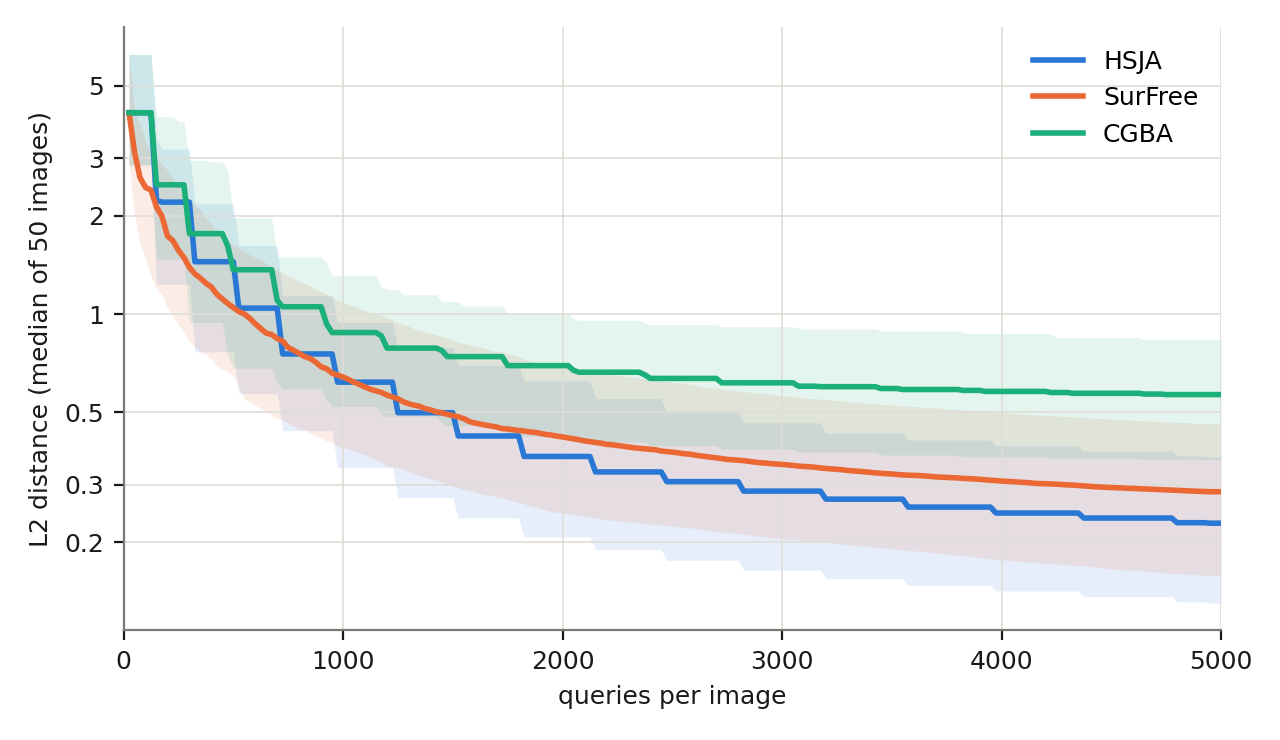
\includegraphics[width=0.5\textwidth]{l2_vs_queries.png}
\caption{Median L2 against queries over the 50 study images, with the interquartile range shaded. SurFree is ahead for the first 700 or so queries; HSJA overtakes it and keeps improving.}
\label{fig:curve}
\end{figure}


\subsection{Changes on top of HSJA}

We then tested changes to HSJA one at a time, each on top of the ones we had kept, on the same 50 images at 5000 queries (table~\ref{tab:study}). The ``holds'' column counts images that stay adversarial under TF32 on the GPU and on the CPU; ``jitter'' is the share that stay adversarial under ten random $\pm$1/255 changes to 5\% of the pixel values, which we use as a cheap proxy for how far past the boundary an image sits.

\begin{table}[tbp]
\centering
\small
\tabStudy
\caption{The ablation study. Success was 100\% in every row. Low-frequency probes and the multi-start variant make L2 worse or no better. Texture weighting raises SSIM by 0.001 and costs L2. The margin trades a little L2 for a large gain in robustness.}
\label{tab:study}
\end{table}

Restricting the probes to the lowest 16$\times$16 or 8$\times$8 DCT frequencies made things clearly worse, \nLowA{} and \nLowB{} against \nStudyBaseLc. We had expected smooth noise to help, as it does on large ImageNet images. A 32$\times$32 image has so few degrees of freedom that discarding most of them probably removes directions the attack needs, but we did not try intermediate sizes.

Trying several starting points worked as designed in the narrow sense: the closest of ten candidates had a mean L2 of 3.606 against 4.643 for the single start, and was closer for 17 of the 50 images. After 5000 queries the final L2 was \nMulti, no better than \nStudyBaseLc. Our reading is that HSJA forgets its start. After a few dozen iterations the current point has moved along the boundary and the original starting direction no longer matters much.
Texture-weighted probes with $p=1$ gave an SSIM of 0.9979 against 0.9969 but raised L2 from \nStudyBaseLc{} to \nTexB, about 27\%, and more than doubled L$_\infty$ (0.025 to 0.058). We kept it because our rule at the time put SSIM first. We now think that was the wrong call if the hidden metric is L2 or L$_\infty$, and dropping it should bring the final L2 back near 0.3. We have not re-run the full 1000 images without it, so that number is an expectation from the 50-image study and not a result.

The 5\% margin is the one change we are confident in. With a 0\% margin, only \nMarginZeroHolds{} of 50 images stayed adversarial on every precision and device, and \nMarginZeroJit\% survived the jitter test. With 5\% all 50 held and \nMarginFiveJit\% survived, for an L2 cost of about 5\% over no margin (\nMarginFiveLc{} against 0.362).

\section{Bugs that cost us time}

\paragraph{TF32 made labels depend on batch size.} PyTorch on Ampere and newer GPUs runs convolutions in TF32 by default. Our first HSJA runs scored 90\%, 95\% and 95\% success at the three budgets on images that, when we checked them afterwards, looked fine. Re-evaluating the saved PNGs under different batch sizes showed that points right at the boundary received different labels depending on whether they were evaluated alone, in a batch of 20, or in a batch of 1020: seven label disagreements across the 60 images we checked. A binary search on a boundary that moves with the batch size is not a binary search. We now run the oracle with TF32 off, and only use TF32 as one of the verification contexts at the end. With it off, the same images produced zero disagreements on the GPU and the CPU.

\paragraph{\texttt{astype(uint8)} truncates.} Our first save function multiplied by 255 and cast. With a perturbation of exactly zero, 426\,197 of the 3\,072\,000 pixel values in the 1000 clean images (13.9\%) changed by one level, because $x\cdot 255$ is often just below an integer. Rounding fixed it, and every image the attack tests is now quantised the same way it will be saved.

\paragraph{A binary search that was not monotone.} Our first fix for the rounding problem binary-searched from the HSJA point back toward the original starting point. The decision regions are not convex, and for some images the search slid nearly all the way back: for \texttt{deer\_1}, L2 went from 0.741 to 4.314. Scaling outward along the ray from the clean image through the HSJA point, which is the direction we want to go anyway, removed the problem.

\paragraph{Images that flipped back after saving.} In the final run \nFixed{} of the 1000 images (\texttt{airplane\_95} and \texttt{bird\_15}) were adversarial in FP32 but not under TF32 or on the CPU after being written to disk. The verification step caught both, pushed each 50\% further along its ray, and re-saved. So the 5\% margin does not remove the problem entirely.

\section{Results}

The final submission fools all 1000 images. Table~\ref{tab:main} gives the averages measured on the saved PNGs, and the per-image numbers are in \texttt{results.csv}. We checked the submission in a fresh process, loading the model the way the organisers' cell does and passing all 1000 images in one batch: 1000 of 1000 were misclassified on the GPU and on the CPU.

\begin{table}[tbp]
\centering
\tabMain
\caption{Final submission, 1000 images, 5000 queries per image (\nTotalQueries{} in total). LPIPS uses the AlexNet backbone.}
\label{tab:main}
\end{table}

The averages hide a wide spread (figure~\ref{fig:hist}). The median L2 is \nMedLc, the 90th percentile \nPninety, and the largest \nMaxLc. At the other end the smallest is \nMinLc, which is a change to a handful of pixel values. In L$_\infty$ the median image has a largest per-pixel change of \nLinfMedian/255, and the worst has \nLinfMax/255. \nGtEight{} of the 1000 images have some pixel changed by more than 8/255 and \nGtSixteen{} by more than 16/255. The mean LPIPS is \nLPIPS, but we have no reference for how LPIPS behaves at 32$\times$32 and would not lean on it.

\begin{figure}[tbp]
\centering
\begin{minipage}[t]{0.57\textwidth}\centering
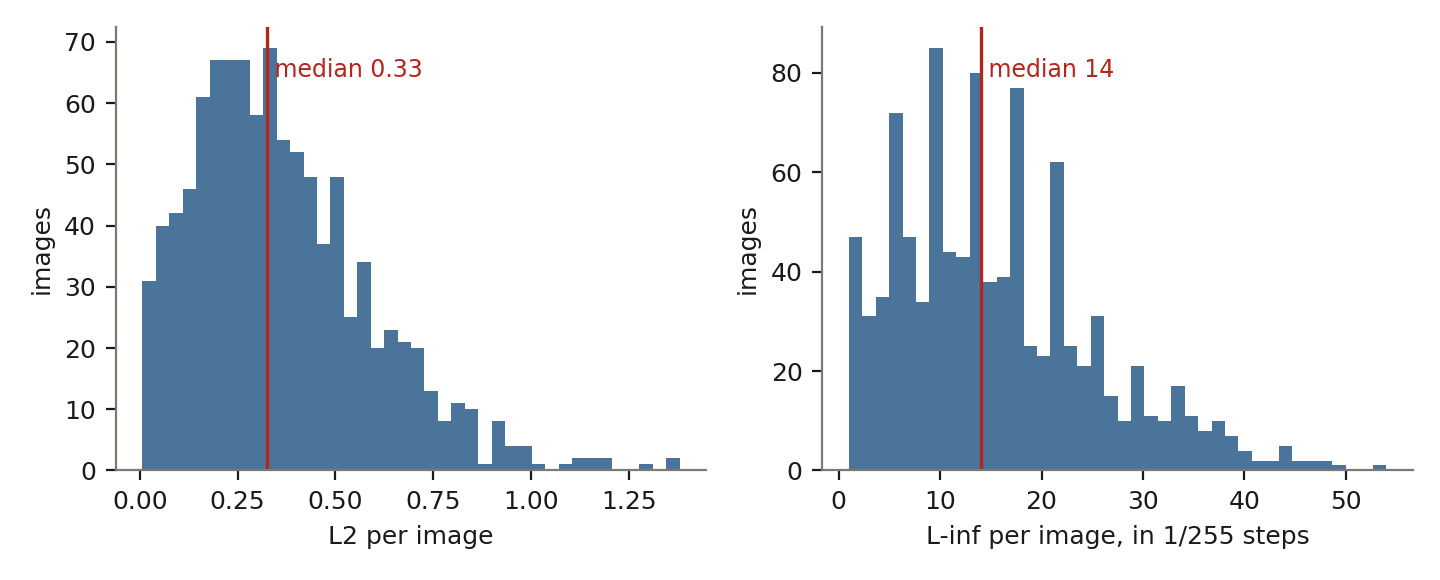
\includegraphics[width=\textwidth]{histograms.png}
\captionof{figure}{Per-image L2 (left) and L$_\infty$ in units of 1/255 (right) for the final submission. The red line marks the median. Both are skewed: most images need little, and a tail needs several times more.}
\label{fig:hist}
\end{minipage}\hfill
\begin{minipage}[t]{0.40\textwidth}\centering
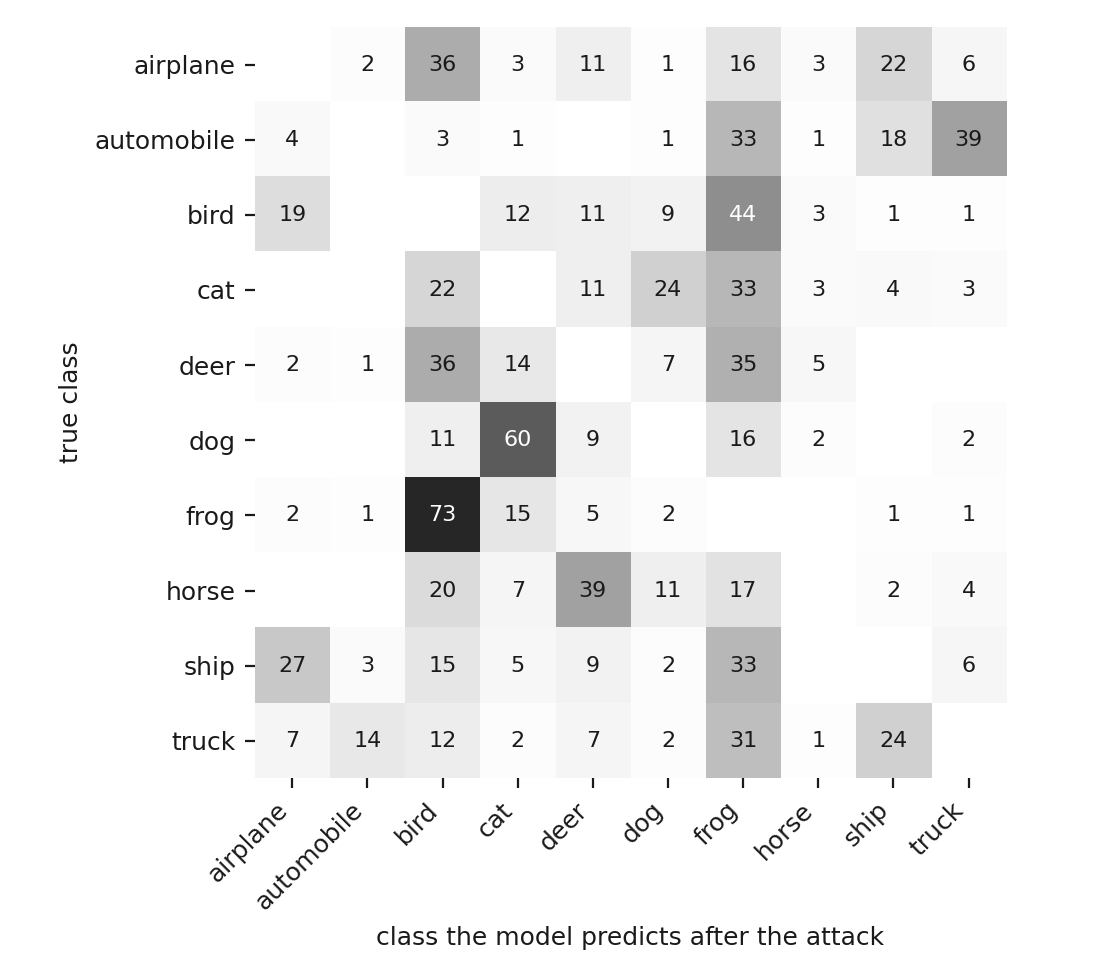
\includegraphics[width=\textwidth]{flips.png}
\captionof{figure}{Class the model predicts after the attack (columns) for each true class (rows), all 1000 images. Rows sum to 100.}
\label{fig:flips}
\end{minipage}
\end{figure}

Figure~\ref{fig:examples} shows the three easiest and three hardest images by L2. The three easiest are animals in dark or low-contrast pictures, where a change that is invisible even when multiplied by ten is enough. The hard ones are the opposite: a bright red truck, a dump truck on white, a rider on a horse, all with sharp edges and saturated colour, and the perturbation has visible structure when magnified. We did not test whether edges and saturation cause the difficulty, so this describes six images and is not a finding.

\begin{figure}[tbp]
\centering
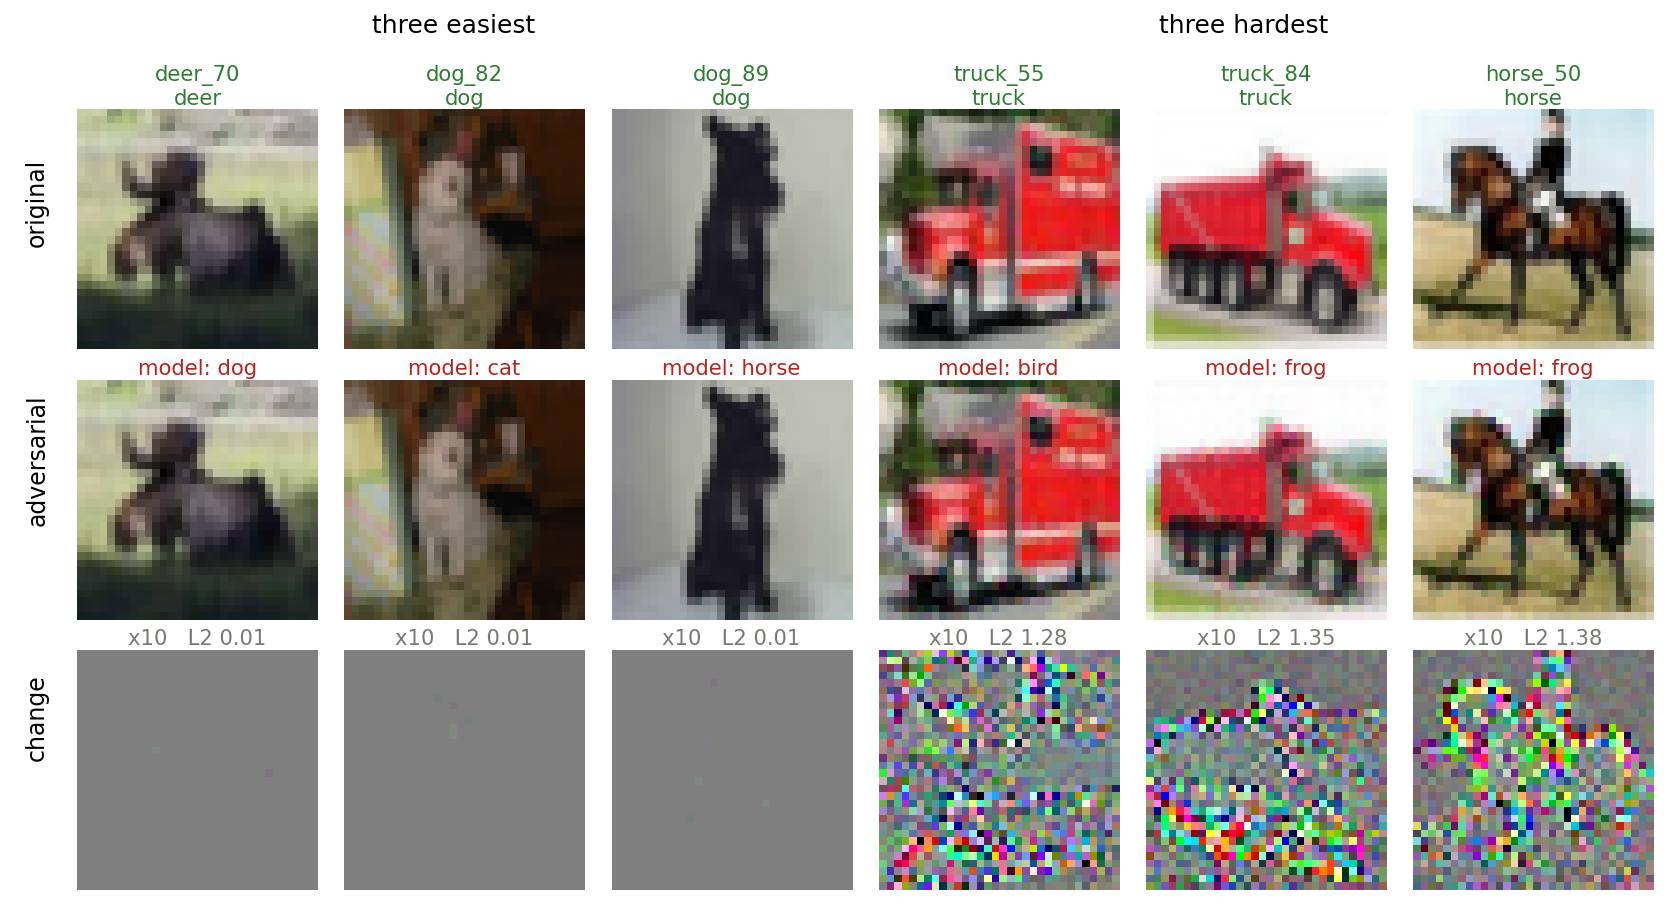
\includegraphics[width=0.68\textwidth]{examples.png}
\caption{Clean image, adversarial image and the difference magnified ten times (grey means no change), for the three easiest and three hardest images by L2. The easiest changes are invisible even at ten times magnification.}
\label{fig:examples}
\end{figure}

The label the model ends up predicting is far from uniform (figure~\ref{fig:flips}). \nTopA{} (\nTopAn) and \nTopB{} (\nTopBn) together account for nearly half the images, followed by \nTopC{} (\nTopCn), while \nBottomA{} (\nBottomAn) and \nBottomB{} (\nBottomBn) are almost never the outcome. We never choose the wrong class, so this reflects where the nearest decision boundary lies for each image together with the starting point: uniform noise is mostly called a bird or a frog by this model, and the walk tends to stay near the region it started in. We have not measured how much of the pattern comes from the start and how much from the boundary geometry.

\section{Limitations and what we would do with more time}

The 50 study images were chosen by taking the first five of each class, not at random, and every ablation number comes from them. With 50 images and a spread like the one in figure~\ref{fig:hist}, differences of a few percent in mean L2 are within noise, so we would not defend the ordering of the close calls (HSJA against HSJA with multi-start, for instance). The large effects, such as low-frequency probes and the 5\% margin, are another matter.

We did not run a targeted version of the attack, and we have no results on whether the label pattern in figure~\ref{fig:flips} can be changed on demand. We also did not try any of the ideas that look promising to us: clipping the largest perturbation values to bring L$_\infty$ down, spending the query budget unevenly so that easy images stop early and hard ones get more, starting from a transfer attack on a public surrogate model, or switching from SurFree to HSJA after the first 700 queries given what table~\ref{tab:compare} shows. The last two use only public models or the labels we already collect, so they would not break the rules, but they are untested, and nothing in this report should be read as evidence for or against them.

The biggest open question remains the metric. If imperceptibility is scored by L2 we should probably drop texture weighting, and if it is scored by SSIM or a perceptual measure we probably should not. We would also check the final images on different hardware, since the TF32 episode shows how easily a label near the boundary can change.

\footnotesize
\setlength{\parskip}{0em}
\begin{thebibliography}{9}
\bibitem{chen2020hsja} J.~Chen, M.~Jordan, M.~Wainwright. HopSkipJumpAttack: a query-efficient decision-based attack. IEEE S\&P, 2020. arXiv:1904.02144.
\bibitem{maho2021surfree} T.~Maho, T.~Furon, E.~Le Merrer. SurFree: a fast surrogate-free black-box attack. CVPR, 2021. arXiv:2011.12807.
\bibitem{reza2023cgba} M.~F.~Reza, A.~Rahmati, T.~Wu, H.~Bayat. CGBA: curvature-aware geometric black-box attack. ICCV, 2023. arXiv:2308.03163.
\bibitem{brendel2018} W.~Brendel, J.~Rauber, M.~Bethge. Decision-based adversarial attacks: reliable attacks against black-box machine learning models. ICLR, 2018. arXiv:1712.04248.
\bibitem{zhang2018lpips} R.~Zhang, P.~Isola, A.~Efros, E.~Shechtman, O.~Wang. The unreasonable effectiveness of deep features as a perceptual metric. CVPR, 2018.
\bibitem{krizhevsky2009} A.~Krizhevsky. Learning multiple layers of features from tiny images. Technical report, 2009.
\end{thebibliography}

\end{document}
